%%%% Thanks to A. Gupta and R. Ravi for providing this template file.



\documentclass[11pt]{article}
\usepackage{amsfonts}
\usepackage{amssymb}
\usepackage{amstext}
\usepackage{amsmath}
\usepackage{xspace}
\usepackage{theorem}
\usepackage{color}
\usepackage[pdftex]{graphicx}
\usepackage{epsfig}
\usepackage[ruled,algosection,vlined,linesnumbered]{algorithm2e}
\usepackage{tikz}
\usepackage{float}
%\usepackage{layout}% if you want to see the layout parameters
                     % and now use \layout command in the body

% This is the stuff for normal spacing
\makeatletter
 \setlength{\textwidth}{6.5in}
 \setlength{\oddsidemargin}{0in}
 \setlength{\evensidemargin}{0in}
 \setlength{\topmargin}{0.25in}
 \setlength{\textheight}{8.25in}
 \setlength{\headheight}{0pt}
 \setlength{\headsep}{0pt}
 \setlength{\marginparwidth}{59pt}

 \setlength{\parindent}{0pt}
 \setlength{\parskip}{5pt plus 1pt}
 \setlength{\theorempreskipamount}{5pt plus 1pt}
 \setlength{\theorempostskipamount}{0pt}
 \setlength{\abovedisplayskip}{8pt plus 3pt minus 6pt}

 \renewcommand{\section}{\@startsection{section}{1}{0mm}%
                                   {2ex plus -1ex minus -.2ex}%
                                   {1.3ex plus .2ex}%
                                   {\normalfont\Large\bfseries}}%
 \renewcommand{\subsection}{\@startsection{subsection}{2}{0mm}%
                                     {1ex plus -1ex minus -.2ex}%
                                     {1ex plus .2ex}%
                                     {\normalfont\large\bfseries}}%
 \renewcommand{\subsubsection}{\@startsection{subsubsection}{3}{0mm}%
                                     {1ex plus -1ex minus -.2ex}%
                                     {1ex plus .2ex}%
                                     {\normalfont\normalsize\bfseries}}
 \renewcommand\paragraph{\@startsection{paragraph}{4}{0mm}%
                                    {1ex \@plus1ex \@minus.2ex}%
                                    {-1em}%
                                    {\normalfont\normalsize\bfseries}}
 \renewcommand\subparagraph{\@startsection{subparagraph}{5}{\parindent}%
                                       {2.0ex \@plus1ex \@minus .2ex}%
                                       {-1em}%
                                      {\normalfont\normalsize\bfseries}}
\makeatother

\newenvironment{proof}{{\bf Proof:  }}{\hfill\rule{2mm}{2mm}}
\newenvironment{proofof}[1]{{\bf Proof of #1:  }}{\hfill\rule{2mm}{2mm}}
\newenvironment{proofofnobox}[1]{{\bf#1:  }}{}\newenvironment{example}{{\bf Example:  }}{\hfill\rule{2mm}{2mm}}
\renewcommand{\thesection}{\lecnum.\arabic{section}}

\renewcommand{\theequation}{\thesection.\arabic{equation}}
\renewcommand{\thefigure}{\thesection.\arabic{figure}}

\newtheorem{fact}{Fact}[section]
\newtheorem{lemma}[fact]{Lemma}
\newtheorem{theorem}[fact]{Theorem}
\newtheorem{definition}[fact]{Definition}
\newtheorem{corollary}[fact]{Corollary}
\newtheorem{proposition}[fact]{Proposition}
\newtheorem{claim}[fact]{Claim}
\newtheorem{exercise}[fact]{Exercise}
\newtheorem{note}[fact]{Note}

% math notation
\newcommand{\R}{\ensuremath{\mathbb R}}
\newcommand{\Z}{\ensuremath{\mathbb Z}}
\newcommand{\N}{\ensuremath{\mathbb N}}
\newcommand{\F}{\ensuremath{\mathcal F}}

\newcommand{\size}[1]{\ensuremath{\left|#1\right|}}
\newcommand{\ceil}[1]{\ensuremath{\left\lceil#1\right\rceil}}
\newcommand{\floor}[1]{\ensuremath{\left\lfloor#1\right\rfloor}}

\DeclareMathOperator{\orb}{orb}


%%%%%%%%%%%%%%%%%%%%%%%%%%%%%%%%%%%%%%%%%%%%%%%%%%%%%%%%%%%%%%%%%%%%%%%%%%%
% Document begins here %%%%%%%%%%%%%%%%%%%%%%%%%%%%%%%%%%%%%%%%%%%%%%%%%%%%
%%%%%%%%%%%%%%%%%%%%%%%%%%%%%%%%%%%%%%%%%%%%%%%%%%%%%%%%%%%%%%%%%%%%%%%%%%%

\newcommand{\headings}[4]{
{\bf CO 759: Topics in Integer Programming} \hfill {{\bf Lecturer:} #1}\\
{{\bf Topic:} #2} \hfill {{\bf Date:} #3} \\
{{\bf Scribe:} #4}\\
\rule[0.1in]{\textwidth}{0.025in}
%\thispagestyle{empty}
}

\begin{document}
\headings{Ricardo Fukasawa}{Orbital Branching, Lattices and Basis Reduction}{Mar/3/2016}{William Justin Toth}
\newcommand{\lecnum}{16}

\section{Orbital Branching}

\paragraph{}
In this section we consider another technique for breaking symmetries while executing Branch and Bound called $\textit{orbital branching}$. As we will see it is very effective at breaking symmetries in some cases. It is even in use in commercial solvers like CPLEX.
\paragraph{}
The setting for this discussion is as follows. Let $P_I = \{x \in \{0,1\}^n : Ax \leq b \}$. Suppose we aim to minimize $c^Tx$ over $x \in P_I$. We will let $\tilde{G}$ denote the formulation group in this context. Suppose we are executing a Branch and Bound algorithm  which wants to branch on $x_j = 0$ or $x_j = 1$ are the root node of the Branch and Bound tree.
\paragraph{}
If we interpret our integer programming problem as modeling some combinatorial problem then fixing $x_j = 0$ is effectively just dropping corresponding object $j$ from solution. This does not gain much, particularly in the face of symmetry, where other variables may take on the role of $x_j$. That is to say, if $x_k \sim x_j$ then fixing $x_j = 0$ does not change much since we have equivalence.
\paragraph{}
Notice there is nothing in the general Branch and Bound procedure forcing us to choose the disjunction $x_j = 0$ or $x_j = 1$ for branching. Any disjunction will do. So let's choose one that better exploits the symmetry. Consider the disjunction
$$ \sum_{k \in \orb(j, \tilde{G})} x_k \leq 0 \text{ or } \sum_{k \in \orb(j, \tilde{G})} x_k \geq 1. $$
\begin{figure}[H]
\centering
\begin{tikzpicture}
\node[shape=circle, draw=black](A) at (0,0) {};
\node[shape=circle, draw=black](B) at (-1,-1){};
\node[shape=circle, draw=black](C) at (1,-1){};

\path[-] (A) edge node[left] { $\sum_{k \in \orb(j, \tilde{G})} x_k \leq 0$}  (B);
\path[-] (A) edge node[right] { $\sum_{k \in \orb(j, \tilde{G})} x_k \geq 1$}  (C);
\end{tikzpicture}
\caption{The Branch and Bound tree with disjunction under consideration}
\end{figure}
\begin{note} The condition $\sum_{k \in \orb(j, \tilde{G})} x_k \leq 0$ is equivalent to saying $x_k = 0$ for all $k \in \orb(j, \tilde{G})$.
\end{note}
\paragraph{}
Another way to interpret $\sum_{k \in \orb(j, \tilde{G})} x_k \geq 1$ is to create one branch fixing each $x_k = 1$ for $k \in \orb(j, \tilde{G})$. 
\begin{figure}[H]
\centering
\begin{tikzpicture}
\node[shape=circle, draw=black](A) at (0,1) {};
\node[shape=circle, draw=black](B) at (-1,-1){};
\node[shape=circle, draw=black](C) at (1,-1){};
\node[shape=circle, draw=black](D) at (5,-1){};
\path[-] (A) edge node[left] { $\sum_{k \in \orb(j, \tilde{G})} x_k \leq 0$}  (B);
\path[-] (A) edge node[right] { $x_{k_1} = 1$}  (C);
\path[-] (A) edge node[right]{$x_{k_l} = 1$} (D);
\path[dashed](C) edge node[below]{$k_1, \dots, k_l$}(D);
\end{tikzpicture}
\caption{The Branch and Bound tree fixing each $x_k = 1$ for $k \in \{k_1, \dots, k_l\} = \orb(j, \tilde{G})$}
\end{figure}
\paragraph{}
But this approach would potentially lead to many branches. Fortunately since
$$x_{k_1} \sim x_{k_2} \sim \dots \sim x_{k_l} $$
branching on each $x_{k_i}$ is equivalent, and we need only branch on $x_j$. Doing this is what is referred to as $\textit{orbital branching}$. Below is a figure visually representing the technique. We will follow with an example demonstrating the effectiveness of orbital branching.
\begin{figure}[H]
\centering
\begin{tikzpicture}
\node[shape=circle, draw=black](A) at (0,0) {};
\node[shape=circle, draw=black](B) at (-1,-1){};
\node[shape=circle, draw=black](C) at (1,-1){};

\path[-] (A) edge node[left] { $x_k = 0$ for all $k \in \orb(j, \tilde{G})$}  (B);
\path[-] (A) edge node[right] {$x_j = 1$}  (C);
\end{tikzpicture}
\caption{The Branch and Bound tree with orbital branching at $x_j$}
\end{figure}
\subsection{Orbital Branching Example}
\paragraph{}
Consider the integer programming formulation of the maximum cardinality stable set problem (given a graph $G=(V,E)$ find a set of vertices with no edges between them as large as possible):
\begin{align*}
&\text{max} &\sum_{v\in V} x_v \\
&s.t. &x_j + x_j &\leq 1, &\text{for all $ij \in E$} \\
& &x_v &\in \{0,1\}, &\text{for all $v \in V$}.
\end{align*}
Suppose we are trying to solve the problem with input graph $G$ draw below:
\begin{figure}[H]
\centering
\begin{tikzpicture}
\node[shape=circle, draw=black](5) at (1,3) {5};
\node[shape=circle, draw=black](12) at (2,3) {12};
\node[shape=circle, draw=black](6) at (0,2) {6};
\node[shape=circle, draw=black](1) at (1,2) {1};
\node[shape=circle, draw=black](4) at (2,2) {4};
\node[shape=circle, draw=black](11) at (3,2) {11};
\node[shape=circle, draw=black](7) at (0,1) {7};
\node[shape=circle, draw=black](2) at (1,1) {2};
\node[shape=circle, draw=black](3) at (2,1) {3};
\node[shape=circle, draw=black](10) at (3,1) {10};
\node[shape=circle, draw=black](8) at (1,0) {8};
\node[shape=circle, draw=black](9) at (2,0) {9};

\path[-] (5) edge (6);
\path[-] (5) edge (1);
\path[-] (1) edge (6);

\path[-] (12) edge (4);
\path[-] (11) edge (4);
\path[-] (12) edge (11);

\path[-] (7) edge (2);
\path[-] (8) edge (2);
\path[-] (7) edge (8);

\path[-] (3) edge (10);
\path[-] (9) edge (10);
\path[-] (3) edge (9);

\path[-] (1) edge (2);
\path[-] (3) edge (2);
\path[-] (3) edge (4);
\path[-] (1) edge (4);
\end{tikzpicture}
\caption{Input graph $G$}
\end{figure}
If we solve the linear programming relaxation we obtain the solution $x_v = \frac{1}{2}$ for all $v \in V$. Let's say our algorithm decides to branch on $x_5$. The branch $x_5 = 1$ is used in both the original branching method and orbital branching. The graph for the subproblem with $x_5 = 1$ is shown below.
\begin{figure}[H]
\centering
\begin{tikzpicture}

\node[shape=circle, draw=black](12) at (2,3) {12};
\node[shape=circle, draw=black](4) at (2,2) {4};
\node[shape=circle, draw=black](11) at (3,2) {11};
\node[shape=circle, draw=black](7) at (0,1) {7};
\node[shape=circle, draw=black](2) at (1,1) {2};
\node[shape=circle, draw=black](3) at (2,1) {3};
\node[shape=circle, draw=black](10) at (3,1) {10};
\node[shape=circle, draw=black](8) at (1,0) {8};
\node[shape=circle, draw=black](9) at (2,0) {9};


\path[-] (12) edge (4);
\path[-] (11) edge (4);
\path[-] (12) edge (11);

\path[-] (7) edge (2);
\path[-] (8) edge (2);
\path[-] (7) edge (8);

\path[-] (3) edge (10);
\path[-] (9) edge (10);
\path[-] (3) edge (9);


\path[-] (3) edge (2);
\path[-] (3) edge (4);
\end{tikzpicture}
\caption{Subproblem for $x_5 = 1$}
\end{figure}
Now the other branch is where we see the difference. If the original branching strategy was used we would have the subproblem shown below.
\begin{figure}[H]
\centering
\begin{tikzpicture}
\node[shape=circle, draw=black](12) at (2,3) {12};
\node[shape=circle, draw=black](6) at (0,2) {6};
\node[shape=circle, draw=black](1) at (1,2) {1};
\node[shape=circle, draw=black](4) at (2,2) {4};
\node[shape=circle, draw=black](11) at (3,2) {11};
\node[shape=circle, draw=black](7) at (0,1) {7};
\node[shape=circle, draw=black](2) at (1,1) {2};
\node[shape=circle, draw=black](3) at (2,1) {3};
\node[shape=circle, draw=black](10) at (3,1) {10};
\node[shape=circle, draw=black](8) at (1,0) {8};
\node[shape=circle, draw=black](9) at (2,0) {9};

\path[-] (1) edge (6);

\path[-] (12) edge (4);
\path[-] (11) edge (4);
\path[-] (12) edge (11);

\path[-] (7) edge (2);
\path[-] (8) edge (2);
\path[-] (7) edge (8);

\path[-] (3) edge (10);
\path[-] (9) edge (10);
\path[-] (3) edge (9);

\path[-] (1) edge (2);
\path[-] (3) edge (2);
\path[-] (3) edge (4);
\path[-] (1) edge (4);
\end{tikzpicture}
\caption{Subproblem for original branching $x_5 = 0$}
\end{figure}
But if we use orbital branching we obtain the much smaller subproblem:
\begin{figure}[H]
\centering
\begin{tikzpicture}
\node[shape=circle, draw=black](1) at (1,2) {1};
\node[shape=circle, draw=black](4) at (2,2) {4};
\node[shape=circle, draw=black](2) at (1,1) {2};
\node[shape=circle, draw=black](3) at (2,1) {3};

\path[-] (1) edge (2);
\path[-] (3) edge (2);
\path[-] (3) edge (4);
\path[-] (1) edge (4);
\end{tikzpicture}
\caption{Subproblem for orbital branching $x_k = 0$ for all $k \in \orb(5,\tilde{G})$}
\end{figure}
This shows the benefits obtained using an orbital branching strategy.
\section{Lattices and Basis Reduction}
\paragraph{}
The goal in this section is an algorithm to determine if $\{x \in \Z^n: Ax=b, 0 \leq x \leq u \} = \emptyset$ (assuming $A$, $b$, and $u$ are integral) in polynomial time for fixed $n$. Meaning we seek an algorithm that may be exponential in $n$, but polynomial in the number of constraints and the size of their values. The naive algorithm is exponential in $u$ (takes $O(u^n) = O(2^{log(n)})$).
\paragraph{}
We begin by considering a simpler question. Let $\mathcal{F} = \{x \in \Z^n: Ax=b \}$. We seek an algorithm that decides if $\mathcal{F} = \emptyset$ in polynomial time for fixed $n$. Notice that we lifted the constraint that $0 \leq x \leq u$. This is a good starting point because a solution may help in solving the more complex problem, and if a solution cannot be found here then we have no hope for the more difficult problem.
\begin{definition}
Let $B = [b_1,\dots,b_d] \in \R^{n \times d}$ be a matrix. Define the lattice generated by $B$ to be:
$$\mathcal{L}(B) := \{y \in \R^n : y = Bv \text{ for some } v \in \Z^d \}.$$
That is, $\mathcal{L}(B)$ is the set of integer combinations of columns of $B$. We call $n$ the dimension of $\mathcal{L}(B)$.
\end{definition}
\begin{definition}
If the columns of $B$ are linearly independent then $B$ is called a basis of $\mathcal{B}$ and $d$ is called the rank of $\mathcal{L}(B)$. If $n=d$ then $\mathcal{L}(B)$ is called a full rank lattice.
\end{definition}
\begin{note}
Now the question $$\mathcal{F} = \emptyset?$$ is equivalent to the question $$b \in \mathcal{L}(B)?.$$ 
\end{note}
\begin{example}
Consider the bases:
\begin{align*}
B_1 = \begin{bmatrix} 1 & 0 \\ 0 & 1 \end{bmatrix},
B_2 = \begin{bmatrix} 1 & 1 \\ 0 & 1 \end{bmatrix},
B_3 = \begin{bmatrix} 2 & 0 \\ 0 & 2 \end{bmatrix}.
\end{align*}
Then $\mathcal{L}(B_1) = \mathcal{L}(B_2) = \Z^2$. So lattices can have multiple different bases. That is, some transformations are permitted to a basis of lattice to obtain another basis. But notice that not all transformations are permitted. For instance $B_3 = 2B_1$ but $\mathcal{L}(B^3) \neq \Z^2$. In fact $$\mathcal{L}(B_3) = \{x \in \Z^2: x_1,x_2 \equiv 0 \text{(mod $2$)} \}.$$
The theorem that follows tells us what types of transformations are permitted to a lattice basis to obtain another basis.
\end{example}
\begin{theorem}
Let $B = \begin{bmatrix} b_1 & \dots & b_d \end{bmatrix}$ be a full rank basis of $n$ dimensional lattice $\mathcal{L}$. Then the following hold:
\begin{enumerate}
\item If $U \in \Z^{d \times d}$ is unimodular (recall unimodular means $|\det(U)| = 1$) then $\bar{B} =BU$ is a basis of $\mathcal{L}$.
\item If $\bar{B}$ is a full rank basis of $\mathcal{L}$ then there exists unimodular $U \in Z^{d \times d}$ such that $\bar{B} = BU$.
\end{enumerate}
\end{theorem}
\begin{proof}
\paragraph{(1)}
We will show $x \in \mathcal{L}(B) \iff x \in \mathcal{L}(\bar{B})$:
\begin{align*}
x \in \mathcal{L}(B) &\iff x = Bv &\text{for some $v \in \Z^d$}\\
&\iff x = BUU^{-1}v \\
&\iff x = \bar{B}(U^{-1}v) \\
&\iff x \in \mathcal{L}(\bar{B}) &\text{since $U^{-1}v \in \Z^d$}.
\end{align*}
Notice that $U \in Z^{d \times d}$ and $|\det(U)| = 1$ so $U^{-1} \in Z^{d \times d}$, and thus $U^{-1}v\in \Z^d$.
\paragraph{(2)}
Let $\bar{B} = \begin{bmatrix} \bar{b_1}& \dots & \bar{b_d} \end{bmatrix}$. As $\mathcal{L}(B) = \mathcal{L}(\bar{B})$, we have that $\bar{b_j} \in \mathcal{L}(B)$ for all $j \in [d]$. Therefore for all $j \in [d]$:
$$\exists u^j\text{, } \bar{b_j} = Bu^j.$$
If we let $U = \begin{bmatrix} u^1 & \dots & u^d \end{bmatrix} \in \Z^{d\times d}$ then
$$ \bar{B} = \begin{bmatrix} \bar{b_1}& \dots & \bar{b_d} \end{bmatrix} = B \begin{bmatrix} u^1 & \dots & u^d \end{bmatrix} = BU. $$
So,
\begin{align*}
\bar{B} = BU &\implies B^{-1}\bar{B} = U \\
&\implies \det(B^{-1}\bar{B}) = \det(U) \\
&\implies \frac{\det(\bar{B})}{\det(B))} = \det(U) \\
&\implies \det(U) \neq 0.
\end{align*}
Similarly, by observing that $b_j \in \mathcal{L}(\bar(B))$ for all $j \in [d]$ we may obtain $\bar{U} \in Z^{d \times d}$ such that
$$B = \bar{B}\bar{U}.$$
From which we can see that $U$ is unimodular as follows:
\begin{align*}
B = \bar{B}\bar{U} &\implies \bar{B}^{-1}B = \bar{U} \\
&\implies (B^{-1} \bar{B})^{-1} = \bar{U} \\
&\implies U^{-1} = \bar{U} \\
&\implies U\bar{U} = I \\
&\implies |\det(U)| = 1 &\text{ as $U, \bar{U} \in \Z^{d\times d}$}.
\end{align*}
\end{proof}
\begin{note}
The previous theorem is still true if $B$ and $\bar{B}$ are not full rank $(n \neq d)$ but this complicates the proof.
\end{note}
\begin{corollary}
If $d= n$ and $B, B'$ are bases of $\mathcal{L}$ then $|\det(B)| = |\det(B')|$.
\end{corollary}
\begin{proof}
There exists unimodular $U$ such that $B = B'U$, and thus $$|\det(B)| = |\det(B')\det(U)| = |\det(B')|$$.
\end{proof}
\begin{note}
From this corollary it makes sense to discuss the determinant of a full rank lattice.
\end{note}
\paragraph{}
If Figure $16.2.8$ below matrices $B = \begin{bmatrix} b_1 & b_2 \end{bmatrix}$ and $B' = \begin{bmatrix} b_1' & b_2' \end{bmatrix}$ are bases of full rank lattice $\mathcal{L}$. 
\begin{figure}[H]
\centering
\begin{tikzpicture}
\draw[fill=lightgray] (0,0) -- (0,3) -- node[above]{$|\det(B)| = \det\mathcal{L}$} (3,3) -- (3,0);
\draw[->] (0,0) -- (0,5);
\draw[->] (0,0) -- (5,0);
\draw[->, line width= 1mm] (0,0) -- node[left]{$b_2$} (0,3);
\draw[->, line width= 1mm] (0,0) -- node[below]{$b_1$} (3,0);

\draw[fill=lightgray] (7,0) -- (7,3) -- (10,6) -- node[right]{$|\det(B')| = \det\mathcal{L}$}(10,3);
\draw[->] (7,0) -- (7,5);
\draw[->] (7,0) -- (12,0);
\draw[->, line width= 1mm] (7,0) -- node[left]{$b_2'$} (7,3);
\draw[->, line width= 1mm] (7,0) -- node[below]{$b_1'$} (10,3);
\end{tikzpicture}
\caption{Shapes have same area.}
\end{figure}
\subsection{Deciding if $\mathcal{F} = \emptyset$}
\paragraph{}
With some elementary ideas out of the way we now return to the question of deciding if $\mathcal{F} = \{x \in \Z^n : Ax = b\}$ is empty. To inspire our approach, consider what we would do if we were trying to solve this problem in the linear case ($x \in \R^n$). If $A$ were full row rank, we could partition $A = \begin{bmatrix} A_B & A_N \end{bmatrix}$ for a basis $B$. Then we have
$$
Ax = b \iff A_Bx_b + A_N x_N = b
$$
so we may set 
$$ x_N = 0 \text{ and } x_B = A_B^{-1}b $$
to solve this problem. Now in the integer case ($x \in \Z^n$) this works only if $A_B^{-1}b$ is integral.
\begin{definition}
Let $A \in \Z^{m \times n}$ be a full row rank matrix. Then $A$ is said to be in integer normal form (INF) if for some non-singular lower triangular $B \in \Z^{m \times m}$ we have
$$ A = \begin{bmatrix} B & 0 \end{bmatrix}.$$
\end{definition}
\begin{theorem}
\begin{enumerate}
\item If $A \in \Z^{m \times n}$ is a full row rank matrix then $A$ can be brought to INF by a sequence of the following operations:
\begin{itemize}
\item exchanging two columns,
\item multiplying a column by $-1$,
\item adding integer multiple of one column to another column.
\end{itemize}
\item There exists a unimodular matrix $U \in \Z^{n \times n}$ such that $$AU = \begin{bmatrix} B & 0 \end{bmatrix}.$$
\end{enumerate}
\end{theorem}
\begin{proof}
\paragraph{(1)}
We proceed by induction on the dimensions of $A$. In the base case, where $A$ is a scalar, the result is trivial. In the inductive case we will aim to show a sequence of the allowed operations will transform $A$ into a matrix of the form:
\begin{align*}
\begin{bmatrix}
\alpha & 0\\
x & \bar{A}
\end{bmatrix}
\end{align*}
for some $\alpha \in \Z$ such that $\alpha \geq 0$, $x \in \Z^{m-1}$, and $\bar{A} \in \Z^{m-1 \times n-1}$ of full row rank. After doing so the result follows by induction.
\paragraph{}
By a sequence of column exchanges (orders the columns) and multiplications of columns by $-1$ (so entries become nonnegative) we can transform $A$ such that
$$a_{1,1} \geq \dots \geq a_{1,n} \geq 0.$$
Let $k = \text{max}\{j \in [n]: a_{1,j} > 0 \}$. Such a $k$ exists since $A$ being full row rank implies $a_{1,1} > 0$. If $k = 1$ then $A$ has been transformed into the desired form and we are done by induction.
\paragraph{}
If $k > 1$ then by applying operations of adding integer multiples of one column to another column we may compute the matrix $A'$ from $A$ such that (let $a_j$ denote column $j$ of $A$):
$$A' = \begin{bmatrix}
a_1 - \floor{\frac{a_{1,1}}{a_{1,2}}}a_2, &\dots, & a_{k-1} - \floor{\frac{a_{1,k-1}}{a_{1,k}}}a_k, &a_k, &\dots, &a_n
\end{bmatrix}
$$
Repeat the entire above process on $A'$.
\paragraph{}
To show this construction terminates consider what happens after the columns of $A'$ (derived from $A$) have been reordered to satisfy
$$a'_{1,1} \geq \dots \geq a'_{1,n} \geq 0 $$
during some iteration. Notice only the first $k$ columns are changed, and each $a'_{1,j} \leq a_{1,j}$, so we know that $\text{max}\{j : a'_{1,j} > 0 \} \leq k$. Then,
\begin{align*}
\sum_{j=1}^{k} a'_{1,j} &\leq \sum_{j = 1}^{k}(a_{1,j} - a_{1,j+1}) +a_{1,k} \\
&= a_{1,1} \\
&< \sum_{j=1}^k a_{1,j}.
\end{align*} 
Since the sums above are strictly decreasing, after a finite number of operations this process will terminate. At which point the resulting matrix will be in the desired form, and by induction the result holds.
\paragraph{(2)}
Each legal operation corresponds to multiplying $A$ by some unimodular matrix. Therefore the desired matrix $U$ can be computed by multiplying the unimodular matrices corresponding to the operations applied to $A$ in the proof of part $(a)$ in the order they were applied (the product of unimodular matrices in unimodular).
\end{proof}
\begin{note}
The constructive nature of the proof shows a method for computing $U$ in polynomial time
\end{note}
\begin{theorem}
Let $A \in \Z^{m \times n}$ be a full row rank matrix. Choose $U \in Z^{n\times n}$ such that $AU = \begin{bmatrix} B & 0 \end{bmatrix}$ is in INF. Then the following hold:
\begin{enumerate}
\item $\mathcal{F} = \emptyset \iff B^{-1}b \in \Z^m$.
\item If $\mathcal{F} \neq \emptyset$ then every element $x \in \mathcal{F}$ is of the form
$$x = U_1 B^{-1}b + U_2z$$
for $z \in \Z^{n-m}$, where $U = \begin{bmatrix} U_1 & U_2 \end{bmatrix}$.
\item $\mathcal{F}_0 = \{x \in \Z^n: Ax=0\}$ is a lattice and $U_2$ is a basis for it.
\end{enumerate}
\end{theorem}
\begin{proof}
See following lecture.
\end{proof}
\begin{note}
The first part of this theorem tells us that the problem of deciding if $\mathcal{F} = \emptyset$ is solvable in polynomial time for a fixed $n$. It is interesting to notice that the simple act of adding the bound $x \geq 0$ makes the problem NP-hard.
\end{note}
\end{document}


